\chapter{SocialFramework}
\label{chapter:SocialFramework}

O SocialFramework é uma \textit{engine} do Rails que ajuda a construir redes sociais com recursos comuns e específicos.

O SocialFramework é dividido em três módulos, que são: usuários, rotas e agendas. No módulo de usuários são providos os principais recursos para usuários, como autenticação, registro e pesquisas. No módulo de rotas o \textit{framework} provê recursos para checar a compatibilidade de rotas. No módulo de agenda são oferecidos recursos para definir agendas de usuários e a compatibilidade de horário entre usuários.

Portanto, o SocialFramework pode ajudar a construir redes sociais genéricas e específicas de um modo rápido e prático e sem se preocupar com problemas recorrentes nestes tipos de sistemas.

\section{Instalação}

A instalação do SocialFramework possui dois passos simples.

Primeiro adicione a seguinte linha no arquivo Gemfile:

\begin{lstlisting}[
    label=listing:Gemfile,
    caption=Gemfile,
    numbers=none,
    language=Ruby,
    basicstyle=\footnotesize\sffamily,
    keywordstyle=\color{red},
    stringstyle=\color{blue},
]
gem 'social_framework'
\end{lstlisting}

Após a adição da \textit{gem} no Gemfile, instale-o executando o seguinte comando:

\begin{lstlisting}[
    label=listing:Install,
    caption=Instalação,
    numbers=none,
    language=Bash,
    basicstyle=\footnotesize\sffamily,
    keywordstyle=\color{red},
    stringstyle=\color{blue},
]
$ bundle install
\end{lstlisting}

Isto irá instalar o SocialFramework na aplicação.

Nas seções a seguir será apresentado o funcionamento do SocialFramework como um \textit{framework} do tipo caixa preta e do tipo caixa cinza, mais especificamente nas seções ~\nameref{sec:primeiros_passos} e \nameref{sec:modulos_socialframework} será apresentado o seu uso como um \textit{framework} caixa preta e na seção \nameref{sec:hotspots} será apresentado o seu uso como um \textit{framework} caixa cinza.

\section{Primeiros passos}
\label{sec:primeiros_passos}

O SocialFramework utiliza o Devise, que é uma solução de autenticação flexível para Rails. Para visualizar a documentação completa do Devise acesse: \url{https://github.com/plataformatec/devise}. A classe de usuário foi implementada no SocialFramework e possui algumas diferenças da classe de usuário padrão do Devise, como a adição do atributo nome e dos relacionamentos dos usuários. As controladoras e \textit{views} do Devise também foram alteradas para adicionar os novos recursos.

Inicialmente, alguns arquivos devem ser adicionado na aplicação para que configurações do SocialFramework e do Devise sejam importadas. Esses arquivos são os \textit{initializers}, o arquivo de internacionalização (i18n) do Devise, as rotas e as \textit{views} de \textit{registration} e \textit{session} para criar e autenticar usuários. Para isso deve-se executar:

\begin{lstlisting}[
    label=listing:generate_social_framework,
    caption=Gerando as configurações do SocialFramework e do Devise,
    numbers=none,
    language=Bash,
    basicstyle=\footnotesize\sffamily,
    keywordstyle=\color{red},
    stringstyle=\color{blue},
]
$ rails generate social_framework:install
\end{lstlisting}

Este comando irá criar o arquivo ``config/initializers/devise.rb'' contendo as configurações do Devise, o arquivo ``config/initializers/social\_framework.rb'' que contem as configurações do SocialFramework, o arquivo i18n do Devise e irá adicionar a rota ``devise\_for'' para mapear as controladoras e \textit{views} do Devise. Com isto a aplicação está preparada para usuar o módulo de usuários com as configurações e comportamentos padrões.

Todas as tabelas do \textit{framework} serão criadas no banco de dados da aplicação. Portanto, para testar a aplicação não se deve esquecer de executar as \textit{migrations}:

\begin{lstlisting}[
    label=listing:migrations,
    caption=Migrations,
    numbers=none,
    language=Bash,
    basicstyle=\footnotesize\sffamily,
    keywordstyle=\color{red},
    stringstyle=\color{blue},
]
$ rake db:create
$ rake db:migrate
\end{lstlisting}

Para acessar a página de autenticação acesse a rota ``/users/sing\_in'', esta página está preparada para autenticar usuários com \textit{email} ou nome de usuário. Para cadastrar um novo usuário deve-se acessar a rota ``/users/sing\_up'', ao criar um novo usuário você estará automaticamente conectado.

Quando se usa o Devise Mailer como o Módulo confirmável é necessário adicionar em seu ambiente as configurações para a ação \textit{mailer}, por exemplo, se estiver no ambiente de desenvolvimento deve-se adicionar as seguintes configurações no arquivo `development.rb'.

\begin{lstlisting}[
    label=listing:mailer,
    caption=Configurações de email,
    numbers=left,
    language=Ruby,
    basicstyle=\footnotesize\sffamily,
    keywordstyle=\color{red},
    stringstyle=\color{blue},
    showspaces=false,
    showstringspaces=false,
]
config.action_mailer.default_url_options = {host: 'localhost', port: 3000}

config.action_mailer.delivery_method = :smtp

config.action_mailer.smtp_settings = {
  address: "smtp.gmail.com",
  port: 587,
  domain: ENV["GMAIL_DOMAIN"],
  authentication: "plain",
  enable_starttls_auto: true,
  user_name: ENV["GMAIL_USERNAME"],
  password: ENV["GMAIL_PASSWORD"]
}
\end{lstlisting}

Pode-se alterar os valores em `domain', `user\_name', e `password' ou criar as variáveis de ambiente locais, isso é indicado para esconder essas informações sigilosas e garantir uma maior segurança. As mesmas configurações são válidas para os ambientes de teste e produção, nos arquivos `test.rb' e `production.rb'.

\subsection{Helpers e filtros das controllers}

O Devise fornece alguns elementos para serem usados nas controladoras e \textit{views}. Para configurar uma controladora com uma autenticação de usuário basta adicionar o seguinte \textit{before\_action}, isto funciona porque o SocialFramework já contem a classe de usuário.

\begin{lstlisting}[
    label=listing:authenticate,
    caption=Requer autenticação de usuário,
    numbers=none,
    language=Ruby,
    basicstyle=\footnotesize\sffamily,
    keywordstyle=\color{red},
    stringstyle=\color{blue},
    showspaces=false,
    showstringspaces=false,
]
before_action :authenticate_user!
\end{lstlisting}

Outros elementos são:

\begin{lstlisting}[
    label=listing:signed_in,
    caption=Verifica se o usuário está logado,
    numbers=none,
    language=Ruby,
    basicstyle=\footnotesize\sffamily,
    keywordstyle=\color{red},
    stringstyle=\color{blue},
    showspaces=false,
    showstringspaces=false,
]
user_signed_in?
\end{lstlisting}

\begin{lstlisting}[
    label=listing:current_user,
    caption=Recupera o usuário logado,
    numbers=none,
    language=Ruby,
    basicstyle=\footnotesize\sffamily,
    keywordstyle=\color{red},
    stringstyle=\color{blue},
    showspaces=false,
    showstringspaces=false,
]
current_user
\end{lstlisting}

\begin{lstlisting}[
    label=listing:user_session,
    caption=Recupera a sessão para este escopo,
    numbers=none,
    language=Ruby,
    basicstyle=\footnotesize\sffamily,
    keywordstyle=\color{red},
    stringstyle=\color{blue},
    showspaces=false,
    showstringspaces=false,
]
user_session
\end{lstlisting}

Após o usuário logar, confirmar a conta ou atualizar a senha o Devise irá procurar por uma caminho \textit{root} para redirecionar. Para alterar esse comportamento padrão, pode-se sobrescrever os métodos ``after\_sing\_in\_path\_for'' e ``after\_sing\_out\_path\_for''.

\subsection{Configuração das modelos}
\label{configuracao_das_modelos}

A classe de usuário no SocialFramework implementa os módulos padrões do Devise. Na documentação completa do Devise é possível encontrar todos os módulos e suas características.

Além dos módulos do Devise, a classe de usuário do SocialFramework possui métodos quem implementam os comportamentos para os relacionamentos de usuários. É possível sobrescrever qualquer comportamento extendendo a classe em outra modelo, como:

\begin{lstlisting}[
    label=listing:extensao_user_class,
    caption=Extensão da classe de usuário,
    numbers=none,
    language=Ruby,
    basicstyle=\footnotesize\sffamily,
    keywordstyle=\color{red},
    stringstyle=\color{blue},
    showspaces=false,
    showstringspaces=false,
]
class OtherUserClass < SocialFramework::User
  # Your code goes here
end
\end{lstlisting}

É necessário mudar o nome da classe no arquivo ``routes.rb'' para a nova classe criada, assim o Devise poderá enxergar a nova classe. Para fazer isso:

\begin{lstlisting}[
    label=listing:devise_new_user_class,
    caption=Configurando a nova classe de usuário para o Devise,
    numbers=none,
    language=Ruby,
    basicstyle=\footnotesize\sffamily,
    keywordstyle=\color{red},
    stringstyle=\color{blue},
    showspaces=false,
    showstringspaces=false,
]
devise_for :users, class_name: 'OtherUserClass',
    controllers: {sessions: 'users/sessions',
                  registrations: 'users/registrations',
                  passwords: 'users/passwords'}
\end{lstlisting}

\subsection{Configuração das migrations}
\label{configuracao_das_migrations}

A classe de usuário fornece como padrão os atributos nome de usuário, e-mail e senha. Para adicionar ou remover atributos para esta ou qualquer outra classe pode-se adicionar a \textit{migrate} na aplicação. O SocialFramework dispõe de um gerador para fazer isso, neste caso só é necessário executar:

\begin{lstlisting}[
    label=listing:generate_migrate,
    caption=Geração das migrations,
    numbers=none,
    language=Bash,
    basicstyle=\footnotesize\sffamily,
    keywordstyle=\color{red},
    stringstyle=\color{blue},
    showspaces=false,
    showstringspaces=false,
]
$ rails generate social_framework:install_migrations -m users
\end{lstlisting}

A \textit{migrate} de usuário será adicionada na aplicação e poderá ser alterada. O parâmetro `m' é usado para gerar \textit{migrations} específicas, o \textit{script} espera os nomes das \textit{migrations}. Caso não exista a \textit{migration} na aplicação, esta será gerada.

Caso seja adicionado ou removido um atributo para o usuário deve-se notificar o Devise, usando um filtro \textit{before} na ``ApplicationController'':

\begin{lstlisting}[
    label=listing:user_attribute,
    caption=Configuração para adicionar um novo atributo de usuário,
    numbers=none,
    language=Ruby,
    basicstyle=\footnotesize\sffamily,
    keywordstyle=\color{red},
    stringstyle=\color{blue},
    showspaces=false,
    showstringspaces=false,
]
class ApplicationController < ActionController::Base
  before_action :configure_permitted_parameters, if: :devise_controller?

  protected

  def configure_permitted_parameters
    devise_parameter_sanitizer.for(:sign_up) << :new_attribute
    devise_parameter_sanitizer.for(:account_update) << :new_attribute
  end
end
\end{lstlisting}

Isto faz com que o \textit{sign\_up} e o \textit{account\_update} receba o novo atributo. Pode-se usar o método de remoção para remover os atributos existentes. Para adiconar ou remover o parâmetor em outras ações, por exemplo o \textit{sign\_in}, deve-se fazer o mesmo procedimento.

\subsection{Configuração das controllers}

Todas as controladoras do Devise podem ser extendidas e ter o seus métodos sobrescritos. Por exemplo:

\begin{lstlisting}[
    label=listing:extensao_controller,
    caption=Extensão de uma controller,
    numbers=none,
    language=Ruby,
    basicstyle=\footnotesize\sffamily,
    keywordstyle=\color{red},
    stringstyle=\color{blue},
    showspaces=false,
    showstringspaces=false,
]
class OtherRegistrationControllerClass < Users::RegistrationsController
  # Your code goes here
end
\end{lstlisting}

Outras controladoras são: ``confirmations'', ``omniauth\_callbacks'', ``passwords'', ``sessions'' e ``unlocks''. Para usar os módulos de ``omniauth\_callbacks'', ``unlocks'' e ``confirmations'' é necessário adicionar esses respectivos módulos do Devise na aplicação. Todas as controladoras do Devise no SocialFramework possuem o prefixo ``Users''.

\subsection{Configuração das rotas}

Quando se substitui algumas controladoras do Devise deve-se definir essas novas controladoras nas rotas. Isto pode ser feito alterando o caminho para a controladora na configuração \textit{devise\_for}, como no exemplo a seguir:

\begin{lstlisting}[
    label=listing:configuracao_controller,
    caption=Configuração de uma controller,
    numbers=none,
    language=Ruby,
    basicstyle=\footnotesize\sffamily,
    keywordstyle=\color{red},
    stringstyle=\color{blue},
    showspaces=false,
    showstringspaces=false,
]
devise_for :users, class_name: 'SocialFramework::User',
  controllers: {sessions: 'users/sessions',
                registrations: 'new_registration_controller_path',
                passwords: 'users/passwords'}
\end{lstlisting}

A controladora de registro foi extendida e a nova controladora foi adicionada nas configurações de rotas do Devise.

\subsection{Configuração das views}

Para adicionar as \textit{views} do Devise na aplicação o SocialFramework possui um gerador para executar esta tarefa, para executa-lo deve-se usar o seguinte comando:

\begin{lstlisting}[
    label=listing:gerar_views,
    caption=Geração das views,
    numbers=none,
    language=Bash,
    basicstyle=\footnotesize\sffamily,
    keywordstyle=\color{red},
    stringstyle=\color{blue},
    showspaces=false,
    showstringspaces=false,
]
$ rails generate social_framework:views
\end{lstlisting}

Para adicionar uma \textit{view} específica deve-se usar o parâmetro `-v' e passar o nome das \textit{views}, como no exemplo a seguir:

\begin{lstlisting}[
    label=listing:gerar_views,
    caption=Geração das views,
    numbers=none,
    language=Bash,
    basicstyle=\footnotesize\sffamily,
    keywordstyle=\color{red},
    stringstyle=\color{blue},
    showspaces=false,
    showstringspaces=false,
]
$ rails generate social_framework:views -v registrations sessions passwords
\end{lstlisting}

Este comando irá adicionar as \textit{views} ``registrations'', ``sessions'' e ``passwords'' na aplicação. As outras \textit{views} são: ``confirmations'', ``mailer'' and ``unlocks''. Inicialmente, o SocialFramework adiciona as \textit{views} ``registrations'' e ``sessions'' na aplicação fornecendo autenticação e registro para os usuários.

\section{Módulos do SocialFramework}
\label{sec:modulos_socialframework}

Atualmente o SocialFramework possui os módulos de usuário, de rotas e de agendas. Que serão detalhados a seguir.

\subsection{Módulo de usuários}

Este módulo fornece a lógica principal à redes sociais, como criar, confirmar e remover relacionamentos entre os usuários, além de buscas, registros, atualizações e autenticações.

A estrutura de relacionamentos foi construída com um relacionamento de muitos para muitos entre usuários através de arestas. As aresta possuem o usuário de origem, o usuário de destino, o \textit{status}, pode estar ativo ou inativo, se é bidirecional ou não, que  especifica relacionamentos como bidirecional ou unidirecional, e um rótulo com o nome do relacionamento. Pode-se existir múltiplos relacionamentos entre os mesmos usuários. Cada relacionamento é representado com uma aresta.

Para criar um novo relacionamento entre dois usuários deve-se utilizar o método `create\_relationship' definido na classe de usuário. Esse método possui a seguinte assinatura:

\begin{lstlisting}[
    label=listing:create_relationship,
    caption=Método para criar relacionamento,
    numbers=none,
    language=Ruby,
    basicstyle=\footnotesize\sffamily,
    keywordstyle=\color{red},
    stringstyle=\color{blue},
    showspaces=false,
    showstringspaces=false,
]
create_relationship(destiny, label, bidirectional=true, active=false)
\end{lstlisting}

O usuário que pede o relacionamento deve chamar este método e passar o usuário de destino e rótulo para o relacionamento. Por padrão é criada um relacionamento bidirecional e inativa entre esse usuários. É possível mudar esse comportamento passando os outros parâmetros para o método.

Para ativar o relacionamento criado é necessário uma confirmação. Assim, o de usuário de destino deve invocar o método `confirm\_relationship'. Esse método possui a seguinte assinatura:

\begin{lstlisting}[
    label=listing:confirm_relationship,
    caption=Método para confirmar relacionamento,
    numbers=none,
    language=Ruby,
    basicstyle=\footnotesize\sffamily,
    keywordstyle=\color{red},
    stringstyle=\color{blue},
    showspaces=false,
    showstringspaces=false,
]
confirm_relationship(user, label)
\end{lstlisting}

É necessário passar como parâmetro o usuário de origem e o rótulo com o tipo de relacionamento. O único usuário que pode confirmar o relacionamento é o usuário de destino.

Para remover algum relacionamento, os usuários devem chamar o método `remove\_relationship', passando o outro usuário do relacionamento e o rótulo do relacionamento. Esse método possui a seguinte assinatura:

\begin{lstlisting}[
    label=listing:remove_relationship,
    caption=Método para remover relacionamento,
    numbers=none,
    language=Ruby,
    basicstyle=\footnotesize\sffamily,
    keywordstyle=\color{red},
    stringstyle=\color{blue},
    showspaces=false,
    showstringspaces=false,
]
remove_relationship(destiny, label)
\end{lstlisting}

A classe de usuário fornece também um método para obter os usuários que estão relacionados com um usuário, para isso deve-se invocar o seguinte método:

\begin{lstlisting}[
    label=listing:relationships,
    caption=Método para recuperar usuários com um tipo de relacionamento,
    numbers=none,
    language=Ruby,
    basicstyle=\footnotesize\sffamily,
    keywordstyle=\color{red},
    stringstyle=\color{blue},
    showspaces=false,
    showstringspaces=false,
]
relationships(label, status = true, created_by = "any")
\end{lstlisting}

O rótulo representa com qual tipo de relacionamento se deseja obter os usuários, o \textit{status} é usado para os usuários com relacionamentos ativos ou inativos, o padrão é \textit{true}, o parâmetro `criado por' é usado para especificar qual usuário pode ter criado o relacionamento, caso seja ``any'' qualquer usuário poderá ter criado o relacionamento, caso seja ``self'' os relacionamentos devem possuir como usuário de origem o próprio usuário ou caso seja ``other'' os relacionamentos devem possuir como usuário de destino o próprio usuário.

O módulo de usuários usa um grafo para fornecer algumas funcionalidades, como buscas na rede e sugestão de relacionamentos. Todas estas funcionalidades estão presentes no ``NetworkHelper'' que implementa as classes ``Graph'', ``Vertex'' e ``Edge''. O grafo pode ser acessado a partir do método `graph', que está prensente na classe de usuário. Na ação \textit{sign\_in} o grafo é construido com o usuário logado como \textit{root}. O grafo é construído até a profundidade especificada no \textit{initializer} `social\_framework.rb' na variável `depth\_to\_build', que tem o valor padrão como três. O método `build' possui a seguinte assinatura.

\begin{lstlisting}[
    label=listing:build,
    caption=Método para construir o grafo,
    numbers=none,
    language=Ruby,
    basicstyle=\footnotesize\sffamily,
    keywordstyle=\color{red},
    stringstyle=\color{blue},
    showspaces=false,
    showstringspaces=false,
]
build(root, attributes = [:username, :email, :title], relationships = "all")
\end{lstlisting}

O parametro ``root'' é um usuário que irá ser a raiz do grafo, o parâmetro ``attributes'' corresponde aos atributos de usuário e evento que serão mapeados para os vértices, por padrão contém o nome de usuário, o email e o titulo. O parâmetro ``relationships'' são o tipo de relacionamentos que serão utilizados para a construção do grafo, deve ser uma \textit{string} para especificar um único relacionamento ou um \textit{array} para especificar mais de um relacionamento, caso seja passado a \textit{string} ``any'' o grafo é construido com qualquer relacionamento. Na ação \textit{sign\_in} o grafo é construído com atributos `username', `email' e `title', além de `id'.

Com o grafo construído é possível sugerir relacionamentos. Para isso, utiliza-se o algoritmo ~\nameref{subsec:dfs} para analisar o terceiro nível do grafo e encontrar relacionamentos comuns com o tipo especificado no \textit{initialize} `social\_framework.rb' na variável `relationship\_type\_to\_suggest', que possui o seu valor padrão como ``friend'', a variável `amount\_relationship\_to\_suggest' especifica a quantidade de relacionamentos para fazer a sugestão, o valor padrão é de cinco. Esse método possui a seguinte assinatura.

\begin{lstlisting}[
    label=listing:suggest_relationships,
    caption=Método para sugerir relacionamento,
    numbers=none,
    language=Ruby,
    basicstyle=\footnotesize\sffamily,
    keywordstyle=\color{red},
    stringstyle=\color{blue},
    showspaces=false,
    showstringspaces=false,
]
suggest_relationships(type_relationships = SocialFramework.relationship_type_to_suggest,
  amount_relationships = SocialFramework.amount_relationship_to_suggest)
\end{lstlisting}

Considerando os valores padrão, se um usuário `A' e um usuário `C' tem cinco relacionamento com o tipo de ``friend'' com outros cinco usuários, o sistema irá sugerir ao usuário `A' começar o mesmo relacionamento com o usuário `C'.

A busca no grafo é executado usando o algoritmo ~\nameref{subsec:bfs}. O método da busca possui a seguinte assinatura.

\begin{lstlisting}[
    label=listing:search,
    caption=Método para fazer pesquisa,
    numbers=none,
    language=Ruby,
    basicstyle=\footnotesize\sffamily,
    keywordstyle=\color{red},
    stringstyle=\color{blue},
    showspaces=false,
    showstringspaces=false,
]
search(map, search_in_progress = false, elements_number = SocialFramework.elements_number_to_search)
\end{lstlisting}

É passado um mapa para ser usado na pesquisa, este mapa representa as chaves e valores para comparar com os vértices, por exemplo, o mapa ``\{username: `user', email: `user', title: `event'\}'' fará com que uma pesquisa retorne qualquer vértice que contem a \textit{string} `user' no nome de usuário ou no email ou que contenha a \textit{string} ``event'' no título. O parâmetro `search\_in\_progress' é usado para continuar uma busca para encontrar mais resultados, para continuar deve-se passar \textit{true}. O parâmetro `elements\_number' defini a quantidade de resultados para se retornar, este valor é especificado no \textit{initialize} `social\_framework.rb' na variável `elements\_number\_to\_search', o valor padrão é de cinco.

Um exemplo para continuar uma pesquisa é mostrado a seguir. Por padrão, quando se continua a procurar, o parâmetro `elements\_number' é usado para aumentar o tamanho máximo para os resultados encontrados. Neste caso, a primeira chamada retorna os primeiros cinco elementos encontrados no grafo, a segunda chamada retorna mais dez elementos, totalizando no final quinze elementos. O retorno do método é um hash com duas chaves, a primeira é ``users'' e seu valor é um \textit{array} usuários encontrados, e segunda é ``event'' e seu valor é um \textit{array} de eventos encontrados.

\begin{lstlisting}[
    label=listing:elements_number,
    caption=Exemplo de continuação de pesquisa,
    numbers=none,
    language=Ruby,
    basicstyle=\footnotesize\sffamily,
    keywordstyle=\color{red},
    stringstyle=\color{blue},
    showspaces=false,
    showstringspaces=false,
]
map = {username: 'user', email: 'user', title: 'event'}
graph.search(map)
graph.search(map, true, 10)
\end{lstlisting}

Pode-se alterar o comportamento padrão para continuar pesquisas passando um bloco para o método, este bloco vai indicar como o ``elements\_number'' deve ser aumentado. Por exemplo:

\begin{lstlisting}[
    label=listing:remove_relationship,
    caption=Bloco para aumentar o valor do elements\_number,
    numbers=none,
    language=Ruby,
    basicstyle=\footnotesize\sffamily,
    keywordstyle=\color{red},
    stringstyle=\color{blue},
    showspaces=false,
    showstringspaces=false,
]
map = {username: 'user', email: 'user', title: 'event'}
graph.search(map, false, 1)
graph.search(map, true) { |elements_number| elements_number *= 2 }
\end{lstlisting}


Nesse caso, o `elements\_number' vai dobrar a cada método de pesquisa chamado com esse bloco. Portanto, a primeira chamada retorna um elemento, devido ao valor passado, o segundo dois, a terceira quatro, e assim por diante.

Quando a pesquisa chega ao fim do grafo e ainda não encontrou todos os elementos necessários, uma pesquisa no banco de dados é realizada para completar a \textit{hash}.

\subsection{Módulo de agendas}

Este módulo fornece a lógica para trabalhar com a agenda dos usuários de redes sociais, como criar, inserir, convidar, confirmar, sair e remover eventos.

A estrutura de relacionamentos foi construída do seguinte modo: Uma agenda pertence a um usuário e tem um relacionamento de muitos para muitos com o evento através de um ``Participant\_Event'', o ``Participant\_Event'' tem um atributo confirmado que indica se o usuário confirmou o evento ou se a confirmação está pendente. Além de um evento ser capaz de estar presente em várias agendas, um evento tem um título, uma descrição, uma data e hora de início, uma data e hora de termino, pode ou não ter uma rota associada, e se o evento for particular um outro usuário só poderá participar do evento se for convidado, se não for particular, qualquer usuário pode entrar no evento.

Para criar um novo evento utiliza-se o método `create\_event', definido na classe de agenda. Esse método possuí a seguinte assinatura.

\begin{lstlisting}[
    label=listing:create_evente,
    caption=Método para criar evento,
    numbers=none,
    language=Ruby,
    basicstyle=\footnotesize\sffamily,
    keywordstyle=\color{red},
    stringstyle=\color{blue},
    showspaces=false,
    showstringspaces=false,
]
create_event(title, start, duration = nil, description = "", particular = false)
\end{lstlisting}

Caso não seje passado a duração do evento, a sua descrição ou se é particular, esse terá o seu termino como o final do dia em que o evento ocorrerá, a sua descrição será definida como uma \textit{string} vazia e o evento não será particular. Estas opção poderão ser alteradas passando os respectivos parâmentros na chamada do método. Para o evento ser criado o usuário não poderá ter eventos em sua agenda que choque com o horário do evento que se deseja criar.

Para um usuário entrar em um evento deve-se usar o método `enter\_in\_event', definido na classe de agenda. Este método possui a seguinte assinatura:

\begin{lstlisting}[
    label=listing:enter_in_event,
    caption=Método para entrar em um evento,
    numbers=none,
    language=Ruby,
    basicstyle=\footnotesize\sffamily,
    keywordstyle=\color{red},
    stringstyle=\color{blue},
    showspaces=false,
    showstringspaces=false,
]
enter_in_event(event)
\end{lstlisting}

É necessário passar como parâmetro o evento que o usuário deseja entrar. Para que o usuário consiga entrar no evento, ele não poderá ter eventos em sua agenda que choque com o horário do evento que se deseja entrar.

Para um usuário possa confirmar um convite para entrar em um evento deve-se usar o método `confirm\_event', definido na classe de agenda. Este método possui a seguinte assinatura:

\begin{lstlisting}[
    label=listing:confirm_event,
    caption=Método para confirmar um evento,
    numbers=none,
    language=Ruby,
    basicstyle=\footnotesize\sffamily,
    keywordstyle=\color{red},
    stringstyle=\color{blue},
    showspaces=false,
    showstringspaces=false,
]
confirm_event(event)
\end{lstlisting}

É necessário passar como parâmetro o evento que o usuário deseja confirmar. Para que o usuário consiga entrar no evento, este não poderá ter eventos em sua agenda que choque com o horário do evento que se deseja confirmar.

Para sair de um evento deve-se invocar o método `exit\_event', definido na classe de agenda. Esse método possui a seguinte assinatura:

\begin{lstlisting}[
    label=listing:exit_event,
    caption=Método para sair de um evento,
    numbers=none,
    language=Ruby,
    basicstyle=\footnotesize\sffamily,
    keywordstyle=\color{red},
    stringstyle=\color{blue},
    showspaces=false,
    showstringspaces=false,
]
exit_event(event)
\end{lstlisting}

É necessário passar como parâmetro o evento que o usuário deseja remover da sua agenda. Mas para conseguir sair do evento o usuário não pode ter o papel de `creator' do evento, caso ele seja o criador do evento, este deve passar o papel para outro usuário antes de sair do evento.

Para apagar um evento é necessário invocar o método `remove\_event', definido na classe de agenda. Esse método possui a seguinte assinatura:

\begin{lstlisting}[
    label=listing:remove_event,
    caption=Método para remover um evento,
    numbers=none,
    language=Ruby,
    basicstyle=\footnotesize\sffamily,
    keywordstyle=\color{red},
    stringstyle=\color{blue},
    showspaces=false,
    showstringspaces=false,
]
remove_event(event)
\end{lstlisting}

É necessário passar como parâmetro o evento que se deseja apagar. Mas para conseguir apagar o evento o usuário deve ter o papel de `creator' do evento.

Para verificar se um usuário possui eventos em um intervalo de tempo definido pode-se usar o método `events\_in\_period', definido na classe de agenda. Esse método retorna todos os eventos que estão dentro desse intervalo de tempo e possui a seguinte assinatura:

\begin{lstlisting}[
    label=listing:events_in_period,
    caption=Método para recuperar os eventos dentro de um período de tempo,
    numbers=none,
    language=Ruby,
    basicstyle=\footnotesize\sffamily,
    keywordstyle=\color{red},
    stringstyle=\color{blue},
    showspaces=false,
    showstringspaces=false,
]
events_in_period(start, finish = start.end_of_day)
\end{lstlisting}

Caso não seje passado o final do período como parâmetro, esse terá o seu termino como o final do dia de início.

Para convidar um usuário para um evento deve-se invocar o método `invite', definido na classe evento. Esse método possui a seguinte assinatura:

\begin{lstlisting}[
    label=listing:invite,
    caption=Método para convidar um usuário para um evento,
    numbers=none,
    language=Ruby,
    basicstyle=\footnotesize\sffamily,
    keywordstyle=\color{red},
    stringstyle=\color{blue},
    showspaces=false,
    showstringspaces=false,
]
invite(inviting, guest, relationship = SocialFramework.relationship_type_to_invite)
\end{lstlisting}

É necessário passar como parâmetro o usuário que está convidando e o usuário convidado, caso não seja passado o tipo de relacionameto que os usuários devem possuir será utilizado o tipo definido no arquivo de configuração. Para convidar um usuário para um evento o usuário que convida deve estar confirmado no evento, ter a permissão de `invite' e ter o convidado em seu círculo de relacionamentos com o tipo de relacionamento específicado, deve-se utilizar o tipo `all' para qualquer tipo de relacionamento.

Para alterar o papel de um participante em um evento deve-se invocar o método `change\_participant\_role', definido na classe evento. Esse método possui a seguinte assinatura:

\begin{lstlisting}[
    label=listing:change_participant_role,
    caption=Método para mudar o papel de um usuário,
    numbers=none,
    language=Ruby,
    basicstyle=\footnotesize\sffamily,
    keywordstyle=\color{red},
    stringstyle=\color{blue},
    showspaces=false,
    showstringspaces=false,
]
change_participant_role(maker, participant, action)
\end{lstlisting}

É necessário passar como parâmetro o usuário que irá mudar o papel, o usuário que terá o seu papel alterado e a ação que será executada, esta ação deve ter como prefixo `maker' ou `remove', que indica se será atribuido ou removido um papel, seguido por um `\_' e o papel da ação, por exemplo: `:make\_admin'. Para que a mudança de papel seja realizada com sucesso o usuário que irá mudar o papel deve possuir a permissão de executar a ação. E caso a ação seja `:make\_creator' o usuário que irá mudar o papel receberá o papel de `admin', pois só deve existir um usuário criador do evento.

Para remover um participante de um evento deve-se invocar o método `remove\_participant', definido na classe evento. Esse método possui a seguinte assinatura:

\begin{lstlisting}[
    label=listing:change_participant_role,
    caption=Método para mudar o papel de um usuário,
    numbers=none,
    language=Ruby,
    basicstyle=\footnotesize\sffamily,
    keywordstyle=\color{red},
    stringstyle=\color{blue},
    showspaces=false,
    showstringspaces=false,
]
remove_participant(remover, participant)
\end{lstlisting}

É necessário passar como parâmetro o usuário que irá remover e o usuário que será removido do evento. Para que a remoção seja realizada com sucesso o usuário que irá remover deve ter a permissão de remover um usuário com o papel do usuário que será removido.

Para adicionar uma rota no evento deve-se invocar o método `add\_route', definido na classe evento. Esse método possui a seguinte assinatura:

\begin{lstlisting}[
    label=listing:change_participant_role,
    caption=Método para mudar o papel de um usuário,
    numbers=none,
    language=Ruby,
    basicstyle=\footnotesize\sffamily,
    keywordstyle=\color{red},
    stringstyle=\color{blue},
    showspaces=false,
    showstringspaces=false,
]
add_route(user, route)
\end{lstlisting}

É necessário passar como parâmetro o usuário que irá adicionar a rota no evento e a rota a ser adicionada. Para que a adição seja realizada com sucesso o usuário deve ter a permissão de `:add\_route'.

Para ver todos os usuários do evento, que confirmaram a participção ou não basta chamar o método `users' da classe evento, com a seguinte assinatura:

\begin{lstlisting}[
    label=listing:change_participant_role,
    caption=Método para mudar o papel de um usuário,
    numbers=none,
    language=Ruby,
    basicstyle=\footnotesize\sffamily,
    keywordstyle=\color{red},
    stringstyle=\color{blue},
    showspaces=false,
    showstringspaces=false,
]
users(confirmed = true, role = "all")
\end{lstlisting}

O parâmetro `confirmed' é responsável por determinar se o retorno deve ser dos usuários que confirmaram participação ou não no evento. O parâmetro `role' define o tipo do papel dos usuários no evento, o valor `all' é para todos os papeis.

O módulo de agenda usa um grafo para fornecer os slots de tempo de forma ordenada levando em consideração a maior quantidade de peso dos slots. Essa funcionalidade está presente no módulo `ScheduleHelper', que inclue a classe `ScheduleContext' responsável por invocar os métodos referentes ao módulo de agenda.

Neste grafo os vértices do tipo usuário só possuem ligação com os vértices do tipo slot, e os vértices do tipo slot só possuem ligação com os vértices do tipo usuário, formando assim um grafo bipartido.

Para construir o grafo é necessário incovar o método `build', definido na classe grafo. Esse método possui a seguinte assinatura:

\begin{lstlisting}[
    label=listing:change_participant_role,
    caption=Método para mudar o papel de um usuário,
    numbers=none,
    language=Ruby,
    basicstyle=\footnotesize\sffamily,
    keywordstyle=\color{red},
    stringstyle=\color{blue},
    showspaces=false,
    showstringspaces=false,
]
build(users, start_day, finish_day, start_hour = Time.parse("00:00"), finish_hour = Time.parse("23:59"), slots_size = SocialFramework.slots_size)
\end{lstlisting}

O parâmetro `users' são os usuários que terão suas agendas verficadas a afim de encontrar o melhor horário para uma possível marcação de evento. Este parâmetro pode ser uma \textit{array}, onde nenhum usuário possui peso no evento ou pode ser uma \textit{hash}, onde a chave é o usuário e o valor é o peso de sua presença no evento, este peso tem o seu valor máximo definido no arquivo de configuração na variável `max\_weight\_schedule', caso o usuário tenho o seu peso definido como o símbolo `:fixed' este usuário terá sua presença como obrigatória no evento, e só serão analisados os slots que este usuário possuir disponibilidade.

O parâmetro `start\_day' indica a partir de qual dia o evento poderá ser marcado, e o parâmetro `finish\_day' indica o dia limite para a marcação do evento. O parâmetro `start\_hour' e o parâmetro `finish\_hour' definem o horário de um dia em que o evento poderá ocorrer, por exemplo pode-se definir o horário comercial de 08:00 às 18:00, caso não sejam passados como pâmetro será considerado que o evento poderá ser marcado em qualquer horário.

O parâmetro `slots\_size' indica o tempo de duração dos slots, caso não seja passado como parâmetro é utilizado o tempo padrão, definido no arquivo configuração e com duração de 1 hora.

A quantidade de slots que serão adicionados no grafo depende do intervalo de tempo que se deseja analisar e do tempo de duração de cada slot.

Para criar as arestas entre os usuários e os slots é verificado se o usuário possuim disponibilidade em sua agenda no intervalo de tempo que o slot possui, caso o usuário possua disponibilidade para esse slot é criada uma aresta entre o usuário e o slot, e o peso do usuário é adicionado ao peso do slot. O método retorna os slots ordenados pelo maior peso que cada slot possui.

\subsection{Módulo de rotas}

Este módulo fornece a lógica para trabalhar com rotas. É usado a API do Google Maps para fornecer os alguns recursos para este módulo, como construir uma rota e obter uma localização a partir de uma latitude e uma longitude.

Para um usuário criar uma rota deve-se utilizar o método `create\_route', presente na classe de usuário. A seguir pode-se visualizar a sua assinatura:

\begin{lstlisting}[
    label=listing:create_route,
    caption=Método para criar uma rota,
    numbers=none,
    language=Ruby,
    basicstyle=\footnotesize\sffamily,
    keywordstyle=\color{red},
    stringstyle=\color{blue},
    showspaces=false,
    showstringspaces=false,
]
create_route(title, distance, locations, mode_of_travel = "driving")
\end{lstlisting}


Os parâmetros são o título da rota, a distância que a rota possui e as localizações, que é um \textit{array} com todos os pontos de latitude e longitude para construir rota, a seguir é ilustrado um exemplo do parâmetro \textit{locations}:

\begin{lstlisting}[
    label=listing:locations,
    caption=Exemplo de localizações,
    numbers=none,
    language=Ruby,
    basicstyle=\footnotesize\sffamily,
    keywordstyle=\color{red},
    stringstyle=\color{blue},
    showspaces=false,
    showstringspaces=false,
]
locations = [{latitude: -15.792740000000, longitude: -47.876360000000},
             {latitude: -15.792520000000, longitude: -47.876900000000}]
\end{lstlisting}

E o parâmetro modo de transporte  representa qual o meio de transpote que será utilizado para percorrer a rota, pode ser `driving', `bycicling', `walking' ou `transit', o valor padrão é `walking' para viajar de carro.

Este módulo também fornece um recurso para verificar a compatibilidade entre duas rotas. Para isso deve-se chamar o método `compare\_routes' presente no `route\_helper.rb'.

\begin{lstlisting}[
    label=listing:compare_routes,
    caption=Método para comparar rotas,
    numbers=none,
    language=Ruby,
    basicstyle=\footnotesize\sffamily,
    keywordstyle=\color{red},
    stringstyle=\color{blue},
    showspaces=false,
    showstringspaces=false,
]
compare_routes(principal_route, secondary_route,
          principal_deviation = SocialFramework.principal_deviation,
          secondary_deviation = SocialFramework.secondary_deviation)
\end{lstlisting}

Este método é utilizado para verificar se duas rotas podem ser conectadas em apenas uma rota. O parâmetro `principal\_route' representa a rota que será alterada para auxliar a rota `secondary\_route', se possível. Quando a rota principal não pode ser alterada pode-se tentar alterar a rota secundária para atingir o objetivo. Os parâmetros `principal\_deviation' e `secondary\_deviation' representam um mapa com o modo de transporte e o desvio máximo que rota pode sofrer, o desvio máximo é a distância que uma rota pode ser desviada para atingir o objetivo. Os valores padrões para os desvios das rotas princial e secundária estão presentes no \textit{initialize} `social\_framework.rb' e podem ser alterados.

O método \textit{compare\_routes} retorna um mapa com as informações de compatibilidade, como pode ser visualizado a seguir:

\begin{lstlisting}[
    label=listing:compatible,
    caption=Retorno do método que compara as rotas,
    numbers=none,
    language=Ruby,
    basicstyle=\footnotesize\sffamily,
    keywordstyle=\color{red},
    stringstyle=\color{blue},
    showspaces=false,
    showstringspaces=false,
]
{compatible: false, principal_route: {deviation: :none,
          distance: 0}, secondary_route: {deviation: :none, distance: 0}}
\end{lstlisting}

A chave `compatible' é falsa quando as rotas são incompatíveis ou verdadeira quando são compatíveis. O desvio representa onde a rota poderá ser desviada, pode ser `none', `both', `origin' ou `destiny', e o `distance' é de valor da distância total que a rota possui com o desvio incluso.

As rotas também podem ser relacionadas com eventos. Para fazer o relacionamento deve-se invocar o método `add\_route', presente na classe de evento.

\begin{lstlisting}[
    label=listing:compatible,
    caption=Retorno do método para adicionar uma rota em um evento,
    numbers=none,
    language=Ruby,
    basicstyle=\footnotesize\sffamily,
    keywordstyle=\color{red},
    stringstyle=\color{blue},
    showspaces=false,
    showstringspaces=false,
]
add_route(user, route)
\end{lstlisting}

O primeiro parâmetro é o usuário que tentará adicionar a rota no evento, é necessário que o usuário tenha a permissão `add\_route' no evento (as permissões para executar as ações nos eventos estão definidas no \textit{initialize} `social\_framework.rb'). O segundo parâmetro é a rota que será adicionada no evento. Quando uma rota é adicionada a um evento todos os usuários neste evento recebem essa rota.

\section{Hotspots}
\label{sec:hotspots}

O SocialFramework possui três pontos de \textit{Hotspots} principais, nesses pontos foram implementados três padrões de projeto para auxiliar na estruturação dos elementos do \textit{framework}. Além desses pontos mencionados, o \textit{framework} é todo extensível, e permite ao usuário mudar qualquer comportamento padrão implementado através de heranças e sobrecrita de métodos.

O primeiro Hotspot definido para o \textit{framework} está presente nas classes de modelo. Como mencionada nas sessões \nameref{configuracao_das_modelos} e \nameref{configuracao_das_migrations} é mostrada a possibilidade de se extender uma classe de modelo ou mudar uma \textit{migration} adicionando ou removendos novos atributos para a classe. Porém, existe um problema, quando se extendende uma classe de modelo para sobrescrever algum método padrão essas alterações não serão refletidas para todos os pontos do \textit{framework} onde aquele método é usado. O \nameref{sec:padrao_factory_method} foi usado para resolver esse problema e, com isso agora é possível, usando-se a classe \textit{ModelFabric} dizer qual classe de modelo deve ser construída para ser usada, ou seja, se um usuário do \textit{framework} extender uma classe de modelo qualquer e sobrescrever um de seus métodos, este poderá simplesmente chamar o método estático \textit{get\_class} passando o nome de sua nova classe e essa classe passará a ser usada pelo \textit{framework}. A seguir é apresentado um modelo de uso desse método para melhor entendimento.

\begin{lstlisting}[
    label=listing:get_class,
    caption=Método para construir nova classe de modelo,
    numbers=none,
    language=Ruby,
    basicstyle=\footnotesize\sffamily,
    keywordstyle=\color{red},
    stringstyle=\color{blue},
    showspaces=false,
    showstringspaces=false,
]
ModelFabric.get_class("NovaClasseModelo")
\end{lstlisting}

Existe um outro facilitador desenvolvido no \textit{framework} para trabalhar com o padrão mencionado. Os nomes de todas as classes de modelo estão definidos no \textit{initializer} `social\_framework.rb', sendo assim, quando um desenvolvedor cria uma nova classe de modelo que extende de alguma \textit{model} padrão basta que mude o nome da respectiva classe nesse arquivo e tudo já estará funcionando. Dessa forma, a classe \textit{ModelFabric} se torna transparente para um usuário do \textit{framework} pois está sendo chamada nos métodos internos, e basta fazer a alteração de nome no arquivo `social\_framework.rb', não se esquecendo, que ao se tratar da classe de usuário, que o nome dessa também deve ser alterado no arquivo `routes.rb' para o Devise saber com qual classe de usuário estará trabalhando.

A seguir na figura \ref{padrao_factory_method} pode ser visto o diagrama das classes construídas para aplicação do padrão.

\newpage
\begin{figure}[h]
    \centering
    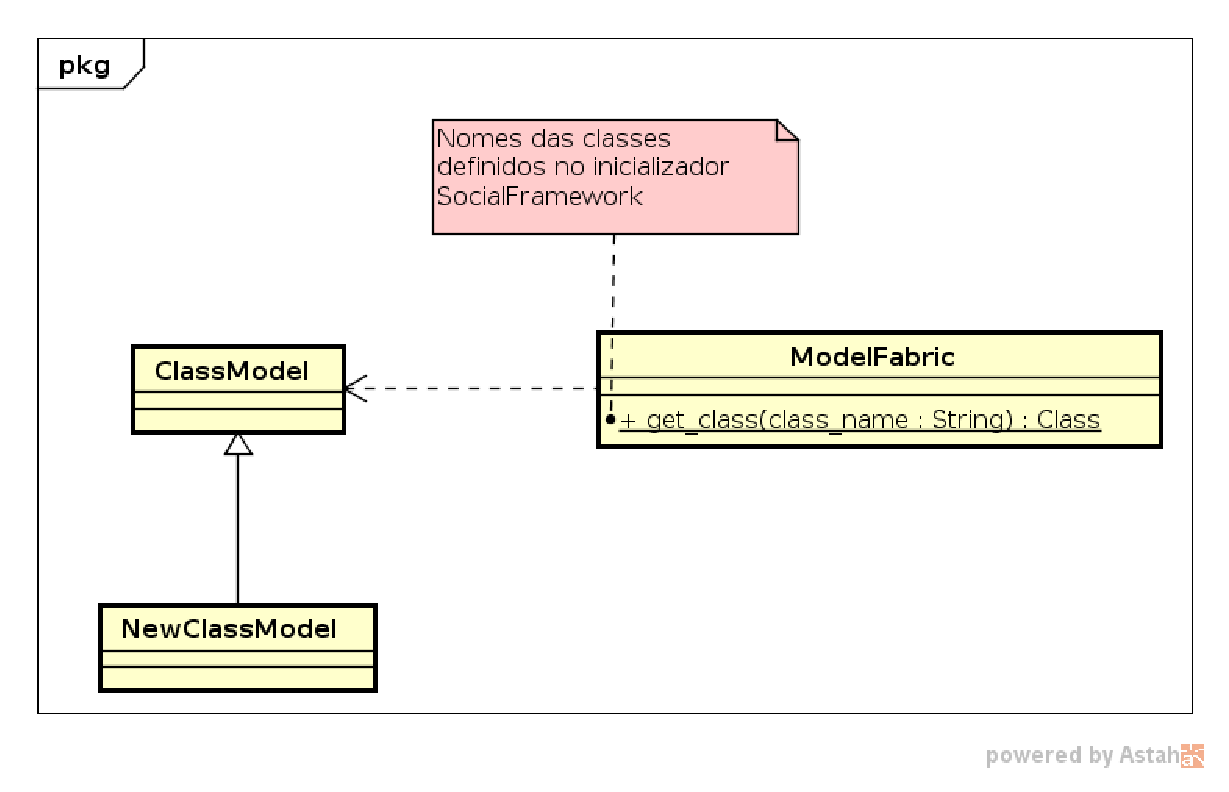
\includegraphics[scale=0.6]{figuras/capitulo6/factory_method.eps}
    \caption{Classes no SocialFramework para aplicação do Factory Method}
    \label{padrao_factory_method}
\end{figure}

Outro padrão de projeto de criação utilizado foi o \nameref{sec:padrao_abstract_factory}. Esse padrão foi utilizado para as classes usadas na construção dos grafos usados na rede de usuários e na conciliação de agendas para marcação de um horário comum. As classe são \textit{Vertex} e \textit{Edge}, para cada um delas existe uma classe abstrata com as assinaturas dos métodos necessários. Também existe a classe abstrata \textit{ElementsFactory} que possui os métodos para criação de Vértices e Arestas.

Para cada classe citada acima foi desenvolvida uma classe concreta que implementa todos os métodos abstrados com o comportamento padrão esperado para eles. As classes são \textit{VertexDefault}, \textit{EdgeDefault} e \textit{ElementsFactoryDefault} que constrói as duas classes anteriores.

Um desenvolverdor com o intuito de alterar qualquer uma das classes \textit{Vertex} ou \textit{Edge} deve extender essas classes e sobrescrever seus métodos conforme sua necessidade, deve-se também extender a classe \textit{ElementsFactory} e sobrescrever os métodos de criação passando suas novas classes. Nas classes que fazem o uso dessas deve ser passado nas instâncias o novo \textit{ElementsFactory} criado e, assim, as novas classes desenvolvidas passarão a ser utilizadas.

O diagrama com as classes construídas no \textit{framework} para aplicação do padrão \textit{Abstract Factory} pode ser visualizado na figura \ref{padrao_abstract_factory}.

\newpage
\begin{figure}[h]
    \centering
    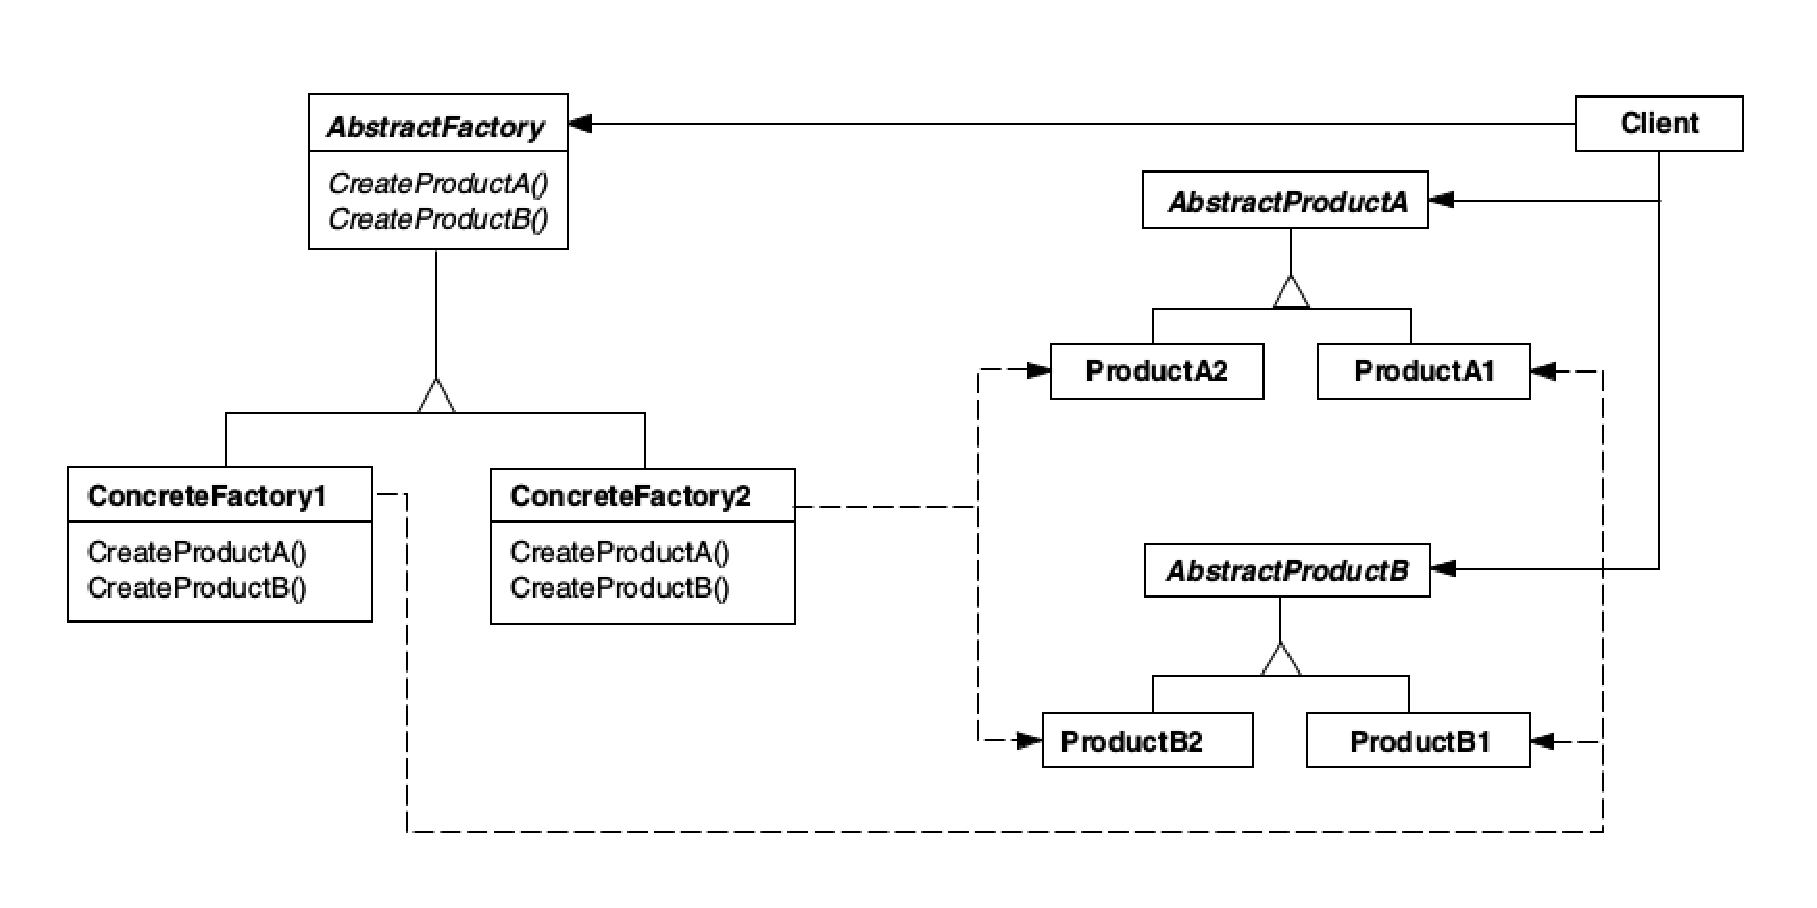
\includegraphics[scale=0.45]{figuras/capitulo6/abstract_factory.eps}
    \caption{Classes no SocialFramework para aplicação do Abstract Factory}
    \label{padrao_abstract_factory}
\end{figure}

No diagrama é mostrado também um exemplo de como seria feita a adição de novas classes que mudem a implementação padrão desenvolvida no \textit{framework}.

Por fim, foi utilizado também o \nameref{sec:padrao_strategy} para cada um dos três módulos do SocialFramework. Para cada um dos módulos existe uma classe abstrata de estratégia que define todos os métodos públicos do módulo e uma classe de contexto que será utilizada pelo usuário do \textit{framework}. Essa classe de contexto que recebe o tipo de estratégia que será utilizado e o \textit{ElementsFactory} quando for alterado.

Por padrão, o SocialFramework já implementa uma classe de estratégia concreta para cada um dos módulos e já recebe essas classes no construtor de cada classe de contexto, porém, é simples para que um desenvolvedor altere a estratégia padrão utilizada, basta que esse crie sua nova classe que extenda da classe abstrata de estratégia do módulo e sobrescreva seus métodos conforme suas necessidades e na instanciação da classe de contexto do módulo deve ser passada a sua nova estratégia construída através do construtor, com isso toda a nova implementação passará a ser usada, sem nenhuma alteração real feita no framework.

Os métodos públicos de cada módulo do SocialFramework que devem ser implementados na mudança de uma estratégia são descritos detalhadamente nas subseções dos \nameref{sec:modulos_socialframework}. As classes de contexto de cada módulo são: \textit{GraphContext} para o módulo de usuário, \textit{ScheduleContext} para o módulo de agenda e \textit{RouteContext} para o móudlo de rotas.

A seguir é apresentado na figura \ref{padrao_strategy} como está a disposição de classes para os três módulos do SocialFramework.

\begin{figure}[h]
    \centering
    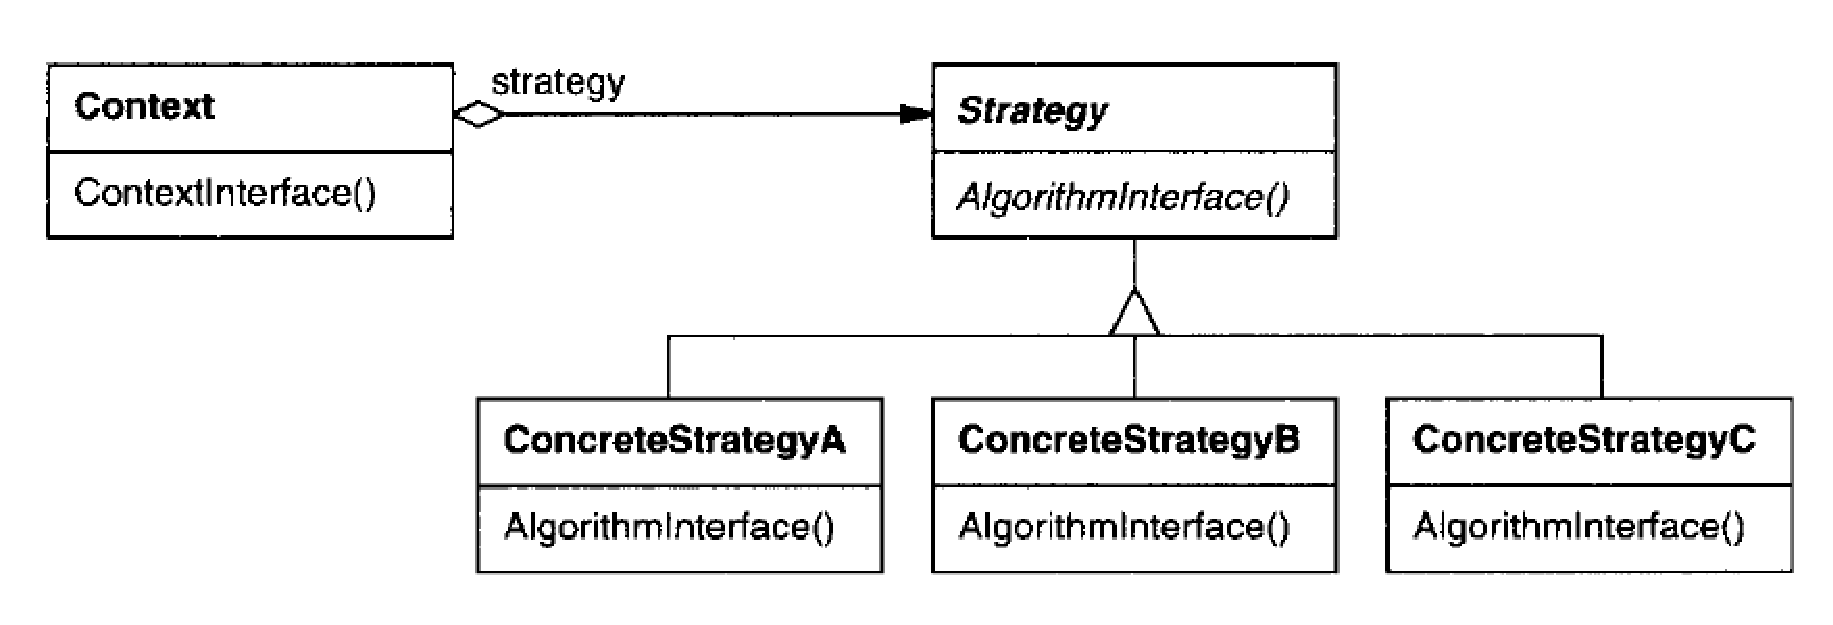
\includegraphics[scale=0.45]{figuras/capitulo6/strategy.eps}
    \caption{Classes no SocialFramework para aplicação do Strategy}
    \label{padrao_strategy}
\end{figure}

Em seguida é apresentado um exemplo de uso quando se altera a estratégia de um módulo.

\begin{lstlisting}[
    label=listing:get_class,
    caption=Instanciação do ScheduleContext quando mudou-se a estratégia,
    numbers=none,
    language=Ruby,
    basicstyle=\footnotesize\sffamily,
    keywordstyle=\color{red},
    stringstyle=\color{blue},
    showspaces=false,
    showstringspaces=false,
]

ScheduleContext.new(NovaEstrategiaDesenvolvida)
\end{lstlisting}

Com isso ao se chamar o método \textit{verify\_availabilities} dessá classe estará chamando de fato o método desenvolvido na class da `NovaEstrategiaDesenvolvida'.

Um exemplo de instancição com alteração da estratégia e também da fábrica de vértices e arestas pode ser visualizado abaixo.

\begin{lstlisting}[
    label=listing:get_class,
    caption=Instanciação do ScheduleContext quando mudou-se a estratégia e a fábrica,
    numbers=none,
    language=Ruby,
    basicstyle=\footnotesize\sffamily,
    keywordstyle=\color{red},
    stringstyle=\color{blue},
    showspaces=false,
    showstringspaces=false,
]

ScheduleContext.new(NovaEstrategiaDesenvolvida, NovaFabricaDeElementos)
\end{lstlisting}

Nesse caso nenhuma das classes padrão do SocialFramework desenvolvidas para serem usadas no módulo de agenda estarão sendo usadas, e sim, as novas classes implementadas pelo usuário do \textit{framework}.
